\documentclass[tikz,border=3pt]{standalone}
\usepackage[utf8]{inputenc}
\usepackage[T1]{fontenc}
\usepackage{lmodern}
\renewcommand{\familydefault}{\sfdefault}
\usepackage{sansmath}\sansmath
\usepackage{chemfig}
\usepackage{pgfplots}\pgfplotsset{compat=1.18,/pgf/number format/use comma,/pgf/number format/1000 sep={.}}
\usetikzlibrary{arrows.meta,calc,positioning,decorations.pathmorphing,patterns}
% paleta del sitio
\definecolor{nar}{HTML}{E8680C}\definecolor{narc}{HTML}{FFB35C}\definecolor{hielo}{HTML}{FFF3E8}
\definecolor{tinta}{HTML}{1D1D1F}\definecolor{gris}{HTML}{6E6E73}\definecolor{lila}{HTML}{7C5CF0}
\definecolor{azul}{HTML}{2F6FD6}\definecolor{menta}{HTML}{17A673}\definecolor{coral}{HTML}{E8342A}
\begin{document}
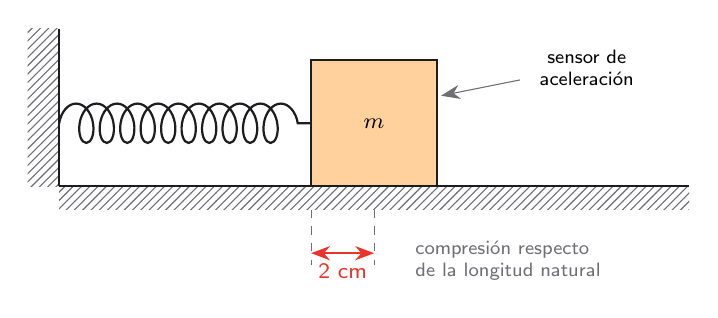
\begin{tikzpicture}[font=\footnotesize,>={Stealth[length=2.4mm]}]
\fill[pattern=north east lines,pattern color=gris] (-0.4,0) rectangle (0,2);
\draw[thick,tinta] (0,0) -- (0,2);
\fill[pattern=north east lines,pattern color=gris] (0,-0.3) rectangle (8,0);
\draw[thick,tinta] (0,0) -- (8,0);
\draw[thick,tinta,decorate,decoration={coil,aspect=0.6,segment length=2.6mm,amplitude=2.5mm}] (0,0.8) -- (3.2,0.8);
\draw[thick,tinta,fill=narc!60] (3.2,0) rectangle (4.8,1.6);
\node at (4,0.8) {$m$};
\draw[dashed,gris] (4.0,-0.3) -- (4.0,-1.0);
\draw[dashed,gris] (3.2,-0.3) -- (3.2,-1.0);
\draw[<->,coral,thick] (3.2,-0.85) -- (4.0,-0.85) node[midway,below] {2 cm};
\node[align=left,anchor=west,text=gris,font=\scriptsize] at (4.4,-0.95) {compresión respecto\\de la longitud natural};
\node[align=center,font=\scriptsize] at (6.7,1.5) {sensor de\\aceleración};
\draw[->,gris] (5.85,1.35) -- (4.85,1.15);
\end{tikzpicture}
\end{document}
